% Graphics for slide 14, in the order the PDF draws them.
\begin{tikzpicture}[remember picture, overlay, x=1bp, y=-1bp,
  shift={(current page.north west)}]
\path[fill=cFFFFFF] (0,0) rectangle (960,540);
\node[anchor=north west, inner sep=0pt] at (56.69,477.21) {
\includegraphics[width=73.42bp, height=37.42bp]{figures/fundamentals-of-hpc/p03-1.png}};
\path[fill=cEE7628,even odd rule] (57.18,55.73) ..controls(57.96,55.73)and(58.6,56.37)..(58.6,57.15) --(58.6,85.5) ..controls(58.6,86.28)and(57.96,86.91)..(57.18,86.91) ..controls(56.4,86.91)and(55.76,86.28)..(55.76,85.5) --(55.76,57.15) ..controls(55.76,56.37)and(56.4,55.73)..(57.18,55.73);
\node[anchor=north west, inner sep=0pt] at (546.32,125.38) {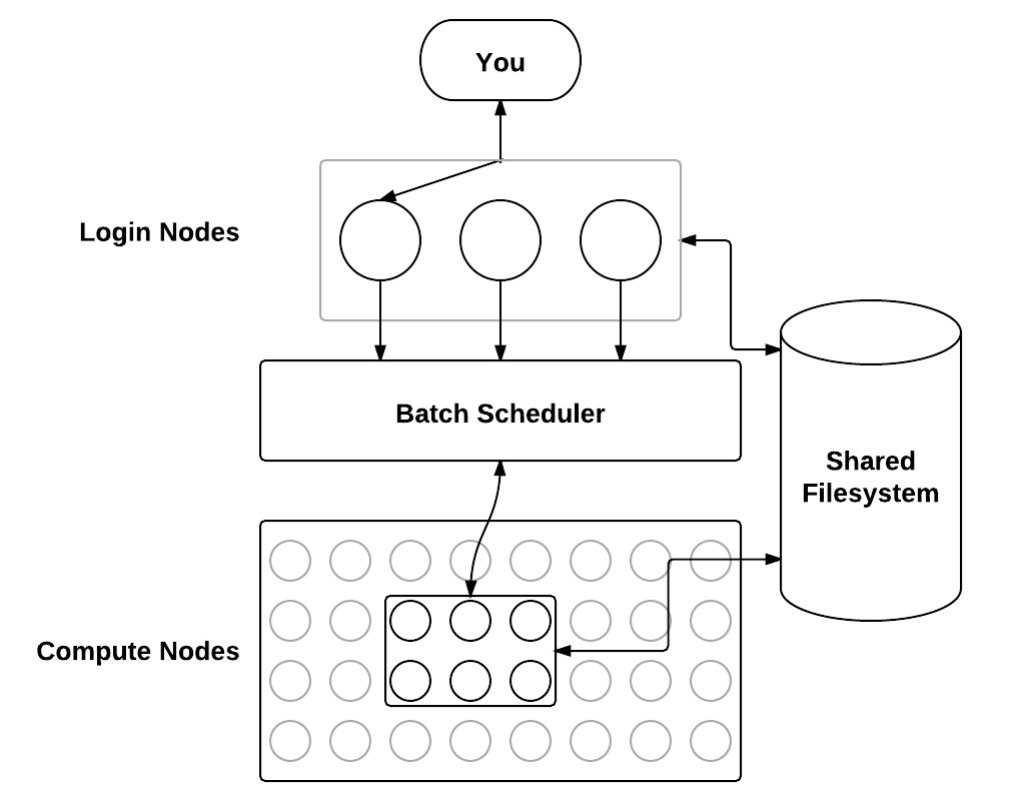
\includegraphics[width=413.68bp, height=319.75bp]{figures/fundamentals-of-hpc/p14-2.jpg}};
\path[fill=cE7303A,even odd rule] (58.6,238.86) ..controls(58.6,234.75)and(61.92,231.43)..(66.03,231.43) --(526.57,231.43) ..controls(530.67,231.43)and(534,234.75)..(534,238.86) --(534,268.57) ..controls(534,272.67)and(530.67,276)..(526.57,276) --(66.03,276) ..controls(61.92,276)and(58.6,272.67)..(58.6,268.57) --(58.6,238.86);
\end{tikzpicture}
